\section{Background}
The main interface of the \HICANNX{} \ASIC{} is a set of $\num{16}$ \LVDS{} lanes. Over these \LVDS{} lanes configuration of the parameters controlling the operation of the chip such as configuration of the synapse connections and the neuron parameters as well as neuron events are transmitted. These neuron events can be inputs from sources external to the \ASIC{} to the network of neurons an synapses aswell as events generaten on the \ASIC{} and transmitted to external sinks.
This communication of events happens in a realtime fashion. The time continuous analog emulation performed by the \ASIC{} cannot be paused and continued arbitrarily. To facilitate this realtime communication a \FPGA{} is used. This thesis will focus mainly on the network attached accelerator deployment. In this case the  \FPGA{} is then connected to a host computer over a network connection. \autoref{fig:schematic_overview} gives a overview over this kind of deployment.
\begin{figure}
\centerline{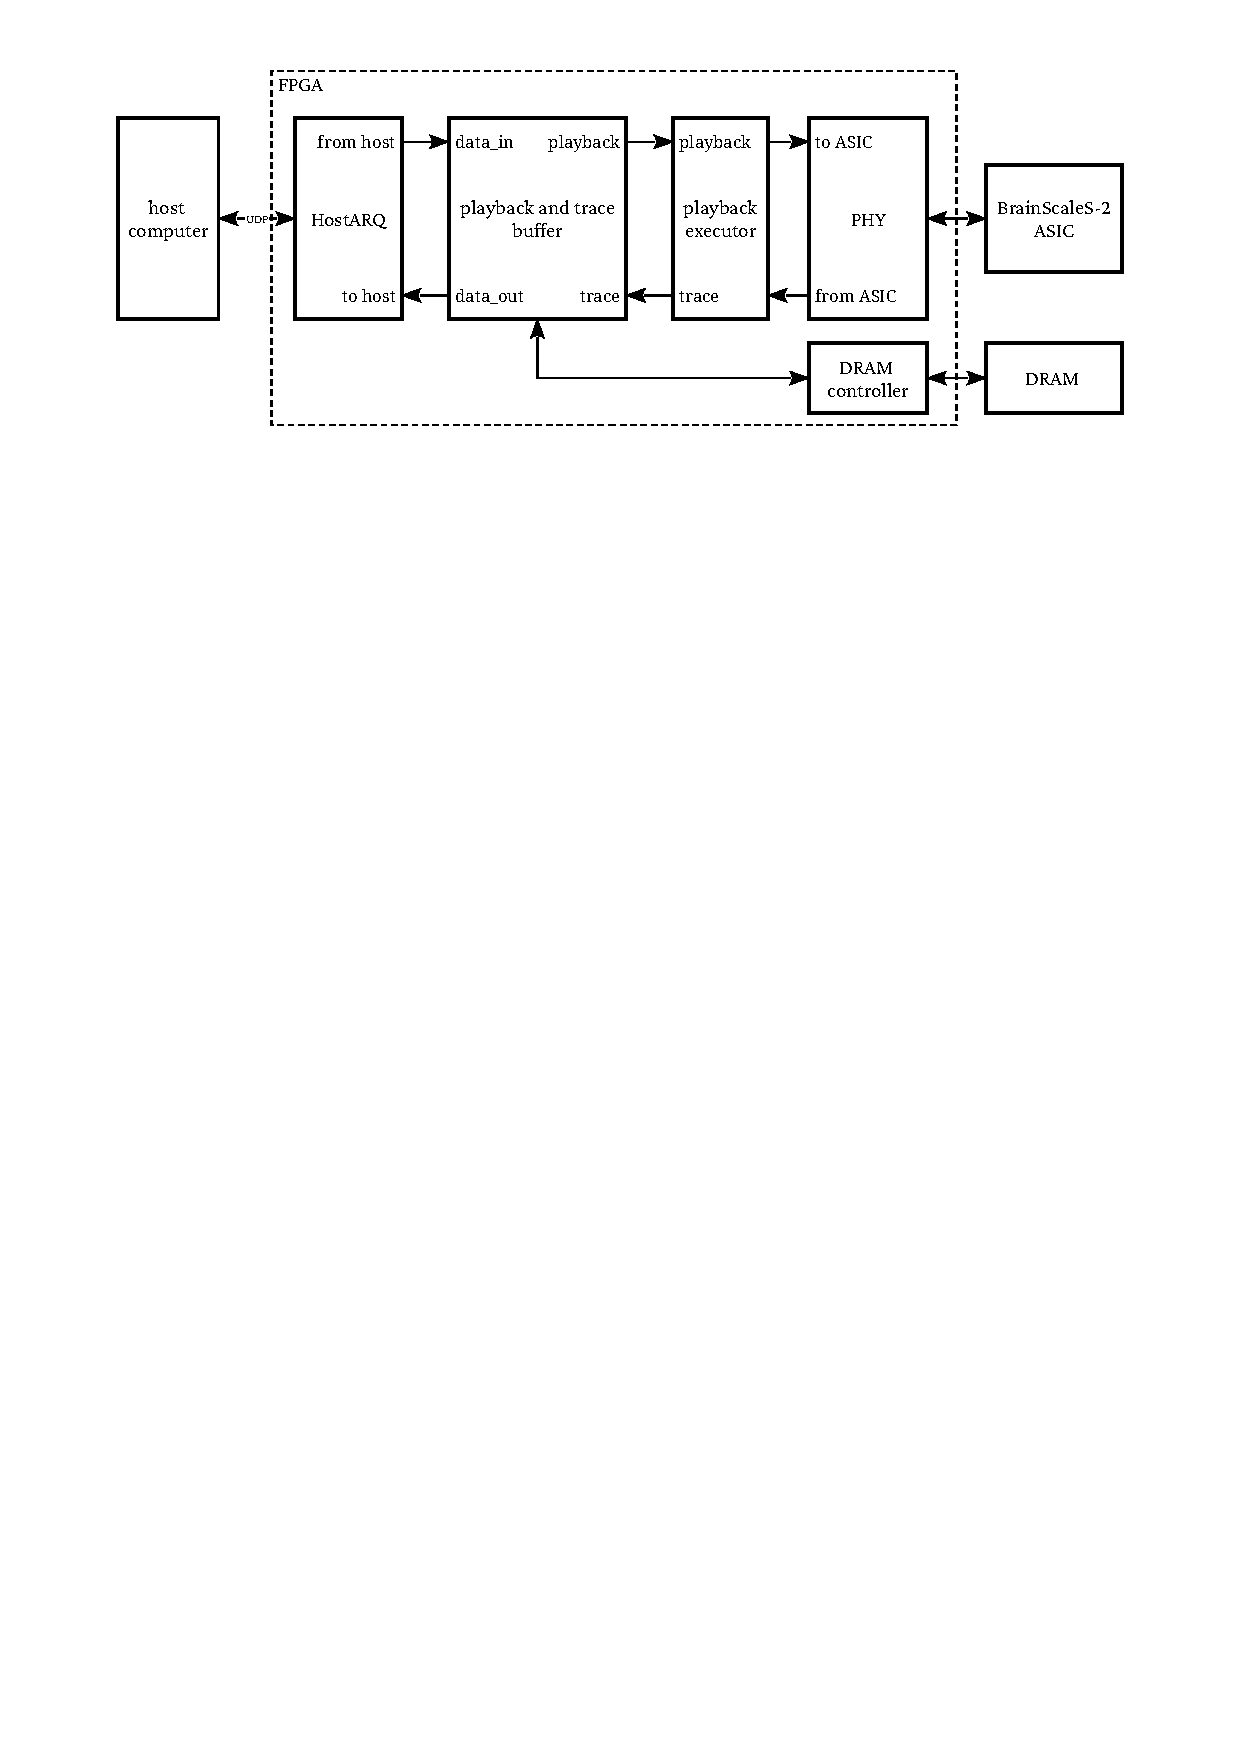
\includegraphics{diagrams/cropped/fpga_overview}}
\caption{Schematic overview of the FPGA design facilitating the communication between a network attached host computer and a \HICANNX{} \ASIC{}. The host computer communicates with the \FPGA{} using the \UDP{} based \HostARQ{} protocol. The \PlaybackProgram{}s received by the \FPGA{} are stored in the playback and trace buffer and executed using the \pbexec{}. Execution by the \pbexec{} generates events that are transmitted to the \ASIC{}. Events received from the \ASIC{} is timestamped by the \pbexec{} and stored in the playback and trace buffer until it is sent to the host.}\label{fig:schematic_overview}
\end{figure}

The realtime communication with the \ASIC{}, especially the transmission and reception of neuron events  requires precise timing and a high bandwidth\autocite{ref:precise_timing}. The precise timing cannot be achieved via the conventional \Gigabitethernet{} used for the communication between \FPGA{} and the host computer.
Instead the \FPGA{} is used to send neuron events to the \ASIC{} with precise timing and timestamp received events. The precise scheduling of event transmission and the timestamping of the received events on the \FPGA{} is performed by the \pbexec{} module on the \FPGA{}.
To perform a experiment the host computer generates a sequence of instructions that among the operations necessary to configure the \ASIC{} includes instructions that contain information about the events and the timing of the events that are to be transmitted to the \ASIC{}. This sequence of instructions, called \PlaybackProgram{}, is then processed by the \pbexec{} with a timing resolution of $\SI{8}{\nano\second}$.
Events received from the \ASIC{} are timestamped with the same resolution.

In the \BSSTwo{}-Cube\autocite{ref:bss_cube} system a \Xilinx{} \Kintex7{} \FPGA{} is used and the \LVDS{} lanes of the \ASIC{} are operated at $\SI{1}{\giga\bit\per\second}$. Moreover the host and the \FPGA{} communicate using \UDP{} protocol over \Gigabitethernet{}. On top of \UDP{} the \HostARQ{}\autocite{ref:hostarq} protocol is used to implement a secured stream with a word size of \PhyWordSize{} over the unsecure \UDP{} protocol.

Because the bandwidth between the host computer and the \FPGA{} is far smaller than the bandwidth between the \FPGA{} and the \ASIC{} the \PlaybackProgram{} as well as the received neuron events need to be buffered by the \FPGA{}. This is aided by the connection of the \FPGA{} to a large external memory.
\autoref{sec:interfaces} and \autoref{sec:pb_exec} give a more detailed overview of the \FPGA{} and especially the \pbexec{}. Finally \autoref{sec:old-pb-trace-management} gives a detailed description of the buffer implementation for the \PlaybackProgram{} and the neuron events, outlines the general requirements for it and highlights its insufficiencies.

This thesis will use these requirements to design a new implementation of the for the \PlaybackProgram{} and the neuron events described in \autoref{sec:impl}.

\todo{explain secured vs unsecured}


\subsection{\AXI{} and stream interfaces}\label{sec:interfaces}
\subsubsection{Stream-Interfaces}
Many components of the \FPGA{} design are connected using stream interfaces. Throughout this thesis two different stream interfaces will be encountered. The first is \AXIStream{}\autocite{ref:axi_stream}, a standard interface used by many components provided by \Xilinx{}.
\AXIStream{} is a unidirectional data stream, that connects a single Transmitter to a single Receiver. A \AXIStream{} consists of at least five signals:
\begin{itemize}
    \item \ACLK{} is the clock signal used by the stream. All other signals will be sampled on the rising edge of this clock.
    \item \ARESETn{} is the reset signal used by the stream. It is active low.
    \item \TDATA{} is the signal carrying the data word. It is a multiple of eight bits wide and driven by the Transmitter.
    \item \TVALID{} is a single bit signal driven by the Transmitter indicating that valid data is present on the \TDATA{} signal.
    \item \TREADY{} is a single bit signal driven by the Receiver indicating that it can accept data.
\end{itemize}
The relation of \TDATA{}, \TVALID{} and \TREADY{} is governed by a set of rules.
Data is transferred from the Transmitter to the Receiver when \TREADY{} and \TVALID{} are driven high simultaneously.
Furthermore a Transmitter is not allowed to wait for the Receiver to drive \TREADY{} high before asserting \TVALID{}. The Receiver, on the contrary, is allowed to wait for the Transmitter to drive \TVALID{} high before asserting \TREADY{}.
When both the Transmitter and the Receiver can process the data fast enough, data can be transferred on every clock cycle. When this is the case \TREADY{} and \TVALID{} will be driven high continuously.
\AXIStream{} defines a set of further signals that can extend the functionality of this stream interface. In this thesis two optional signals will be relevant.
The first is \TKEEP{}. \TKEEP{} has one bit for every eight bits contained in the \TDATA{} signal and is driven by the Transmitter to indicate which bytes of the \TDATA{} signal contain valid data.
If bit $n$ of \TKEEP{} is driven high, bits $8n$ to $8(n + 1) - 1$ of \TDATA{} will contain valid data, if it is driven low the data contained in these bits is to be ignored by the Receiver.
The second optional signal is \TLAST{}. This is a single bit that is driven by the Transmitter which indicates that the current transfer is the last transfer of a packet.

The second stream type encountered in this thesis is used by many of the components of the \FPGA{} that werde developed by this group. In this thesis it will be referred to as \ValidNextStream{}. It is closely related to \AXIStream{}, but replaces the \TREADY{} signal with a \NEXT{} signal.
This is a single bit signal driven by the Reciever to indicate that the current data was processed and the Transmitter can present the next data word on \TDATA{}. Furthermore it has different rules regarding \TVALID{} and \NEXT{} compared to the rules of regarding \TVALID{} and \TREADY{}.
For a \ValidNextStream{} the Transmitter is allowed to wait until the Receiver drives \NEXT{} high before asserting \TVALID{}.

This different rule set means that in general a \AXIStream{} and a \ValidNextStream{} cannot be connected together by simply connecting the \TREADY{} and the \NEXT{} signals as they can deadlock. For example when connecting a \ValidNextStream{} Transmitter to a \AXIStream{} Receiver, the \ValidNextStream{} Transmitter is allowed to wait until the \AXIStream{} Receiver drives \TREADY{} (connected to \NEXT{}) until it drives \TVALID{}. However the \AXIStream{} Receiver is allowed to wait until \TVALID{} is driven high before asserting \TREADY{}. In this case both the Receiver and the Transmitter will wait forever and no progress will be made. This means when connecting a \ValidNextStream{} Transmitter to a \AXIStream{} Receiver, one has to use a \AXIStream{} Receiver that will assert \TREADY{} without waiting until \TVALID{} is asserted by the Transmitter.

\subsubsection{AXI}\label{sec:AXI}
\AXI{}\autocite{ref:axi} is protocol used for communication between some components of the \FPGA{} design. It allows for communication between a single Manager and a Subordinates. It consists of a \ACLK{} and a \ARESETn{} signal that play the same role as they do in a \AXIStream{} as well as five independent channels:
\begin{itemize}
  \item The \AW{} channel transmits information about a write from the Manager to the Subordinate. This information contains the address, the number of words that will be written (the \burstsize{}).
  \item The \AR{} channel transmits information about a read from the Manager to the Subordinate. This information contains the address, the number of words that should be read (the \burstsize{}).
  \item The \W{} channel transmits the data that is written from the Manager to the Subordinate.
  \item The \R{} channel transmits the data that is read from the Subordinate to the Manager.
  \item The \B{} channel transmits a response that contains the result of a write from the Subordinate to the Manager
\end{itemize}
Each of these channels uses the same handshaking signals \READY{} and \VALID{} as well as rules of a \AXIStream{}. Furthermore the \W{} and \R{} channels use a \LAST{} signal to indicate the last word of a burst.

The basic operations of the \AXI{} protocol are read and write transactions. A read transaction is initiated by the Manager by transmitting the address and the number of words that should be read on the \AR{} channel. The subordinate then responds with the corresponding data on the \R{} channel. A write transaction transmits the address that should be written to and the number of words that should be written on the \AW{} channel  and the data that should be written on the \W{} channel. The Subordinate responds with the result of a write transaction one the \B{} channel once it is completed.

Every channel operates separately from each other. This means that for example the data to be written can be transmitted by the Manager on the \W{} channel before the address information is transmitted on the \AW{} channel. A Manager is also allowed to transmit a second read on the \AR{} channel before having received the answer to the first.
From this it follows that the maximum data rate supported by the bus specification is a single data word each clock cycle on both the read and the write channels. The actual data rate depends on the Manager and the Subordinate.

\subsection{Playback Executor}\label{sec:pb_exec}
The \pbexec{} is responsible for processing the instruction stream that is received from the playback and trace buffer as swell as receiving, time stamping and transmission to the playback and trace buffer of events from the \ASIC{}. This section will give a brief overview of this module, a more detail description can be found in \autocite{ref:pb_exec}

The instructions that are processed by the executor can broadly be categorized into the three different categories:
\begin{itemize}
\item Instructions in the \readCat{} perform read operations on the several buses connected to the \pbexec{} and result result in response data that is sent to the trace stream in addition to the events from the \ASIC{}.
\item Instructions of the \writeCat{} perform writes to theses buses.
\item Instructions of the \waitCat{} are used to pause the processing of the instruction stream until a specific event takes place. This can for example be the elapsing of a specific duration or the completion of a read.
\end{itemize}
A special instruction, the \haltInstr{} is used to delineate separate experiments from each other. The \haltInstr{} marks the end of a \PlaybackProgram{} and looped back to the trace data where it can be used to differentiate trace data belonging to different \PlaybackProgram{}s.

There are several sources like the result data of instructions in the \readCat{} and the events received from the \ASIC{} for trace data that is transmitted by the \pbexec{} on the trace stream. The data from these different sources is combined into the single trace stream using a the trace arbiter, which uses a combination of round robin and priority arbitration.

The \pbexec{} operating at a \pbExecClock{} clock rate and can at most process a single instruction every clock cycle, however not every instruction can be processed in a single clock cycle. Obvious examples include instructions of the \waitCat{} which purposefully pause the processing of the instruction stream. Similar to the instruction stream the \pbexec{} can also emit at most a single trace word every clock cycle.

Both the playback instruction stream and the trace data are fundamentally a stream of variable size words. For transmission and reception over the fixed width \HostARQ{} streams they are encoded using \UT{} encoding scheme\autocite{karasenko2020neumann}.

For the playback instruction stream this encoding is performed on the host. On the \FPGA{} the \pbexec{} decodes the instruction stream before processing it.
Likewise the trace data generated / received by the \pbexec{} is encoded by the \pbexec{} before being sent to the trace stream.

The encoding and decoding also operates at a \pbExecClock{} clock rate and can produce / consume at most one \PhyWordSize{} sized word per clock cycle.

This means the maximum data rate at which the playback stream can be processed and the maximum data rate that is sent on the trace stream is
\[\PhyWordSize{} \pbExecClock{} = \pbExecBandwidth{}\]

\begin{figure}
\centerline{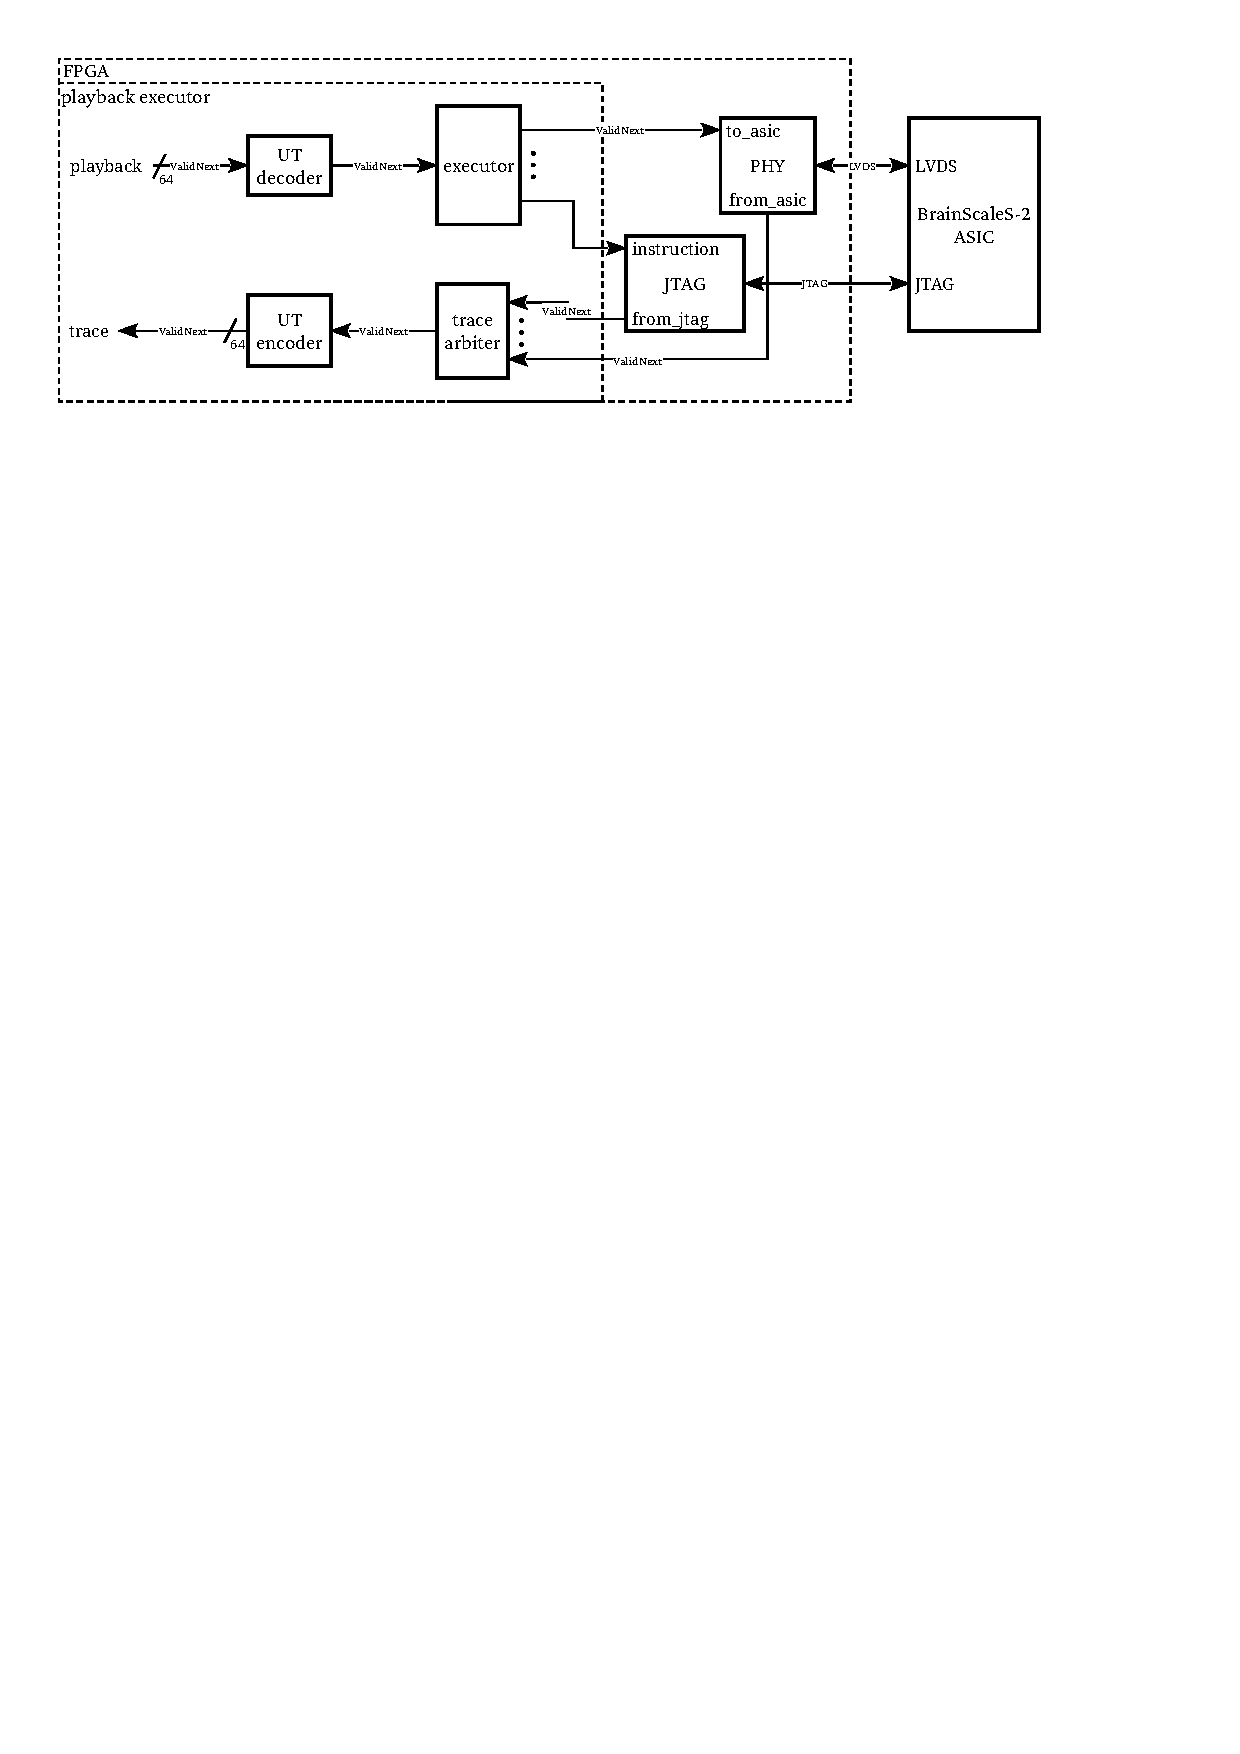
\includegraphics{diagrams/cropped/executor_detail}}
\caption{Overview of the \pbexec{}. The \pbexec{} receives a \UT{} encoded stream of instructions that is decoded by the \UT{} decoder. Each instruction is executed by the executor. Depending on the instruction this can for example cause a event to be sent to the \ASIC{} or a \JTAG{} operation to be performed. Data received from the \ASIC{} as well as data that is for example generated by instructions that read from one of the other \FPGA{} buses is combined into a single variable word width stream by the trace arbiter and encoded into a fixed word width stream by the \UT{} encoder.
This overview is a simplified and does not include all interfaces that the executor has access to and does not include all sources for trace data.}\label{diagram:executor}
\end{figure}

\subsection{Playback and trace buffer}\label{sec:old-pb-trace-management}
The bandwidth between \FPGA{} and the \ASIC{} at \ASICBandwidth{} far exceeds the bandwidth between the host and the \FPGA{} of \HostBandwidth{}. To allow transmission and reception of the full data rate supported between the \FPGA{} and the \ASIC{} the \FPGA{} is connected to \SI{512}{\mebi\byte} of \DDR{} memory that is used as buffer for the playback and trace data.

This section will describe the current implementation of this playback and trace buffer and highlight its shortcomings.

The \FPGA{} design uses the \XilinxMIG{} to allow access to this \DDR{} memory using the \AXI{} protocol.

The playback and trace buffer has two responsibilities:
\begin{itemize}
  \item It stores the playback instructions stream received from the host into the \DDR{} memory and once a complete \PlaybackProgram{} was received reads the \PlaybackProgram{} from the memory and transmits it to the \pbexec{}
  \item It receives the trace data from the \pbexec{} and stores it to the \DDR{} memory until it is transmitted back to the host.
\end{itemize}

In the current \FPGA{} design it operates as a pair of \FIFO{}s. One for the playback stream and one for the trace stream. This \FIFO{} is implemented using the \Xilinx{} \VFIFO{} core, which implements a multi channel \FIFO{} backed by a \AXI{} accessible memory. It is connected to the \AXI{} interface of the \XilinxMIG{}. The \VFIFO{} core is used in a configuration using two channels. The first channel is used for the playback data and the second channel is used for the trace data.

The playback control block is responsible for scheduling the transmission of the playback instruction stream to the \pbexec{}.
It allows data to be transmitted from the \VFIFO{} to the \pbexec{} only  when two conditions are fulfilled:
\begin{enumerate}
\item The \VFIFO{} channel for the playback data is empty or the \FIFO{} between the \VFIFO{} and the \pbexec{} is full
\item The \VFIFO{} channel for the playback data is full or a \haltInstr{} was written to the \VFIFO{} but not transmitted to the \pbexec{}
\end{enumerate}
When a complete \PlaybackProgram{} fits into the \VFIFO{} playback channel, these two conditions enforce that playback of the instructions that make up the \PlaybackProgram{} is only started once it was completely transmitted to the \VFIFO{}, as each \PlaybackProgram{} ends with a \haltInstr{}. This ensures that the rate of instructions that can be transmitted to the \pbexec{} is not limited by the slow \HostARQ{} interface but instead by the \VFIFO{} and indirectly by the \XilinxMIG{} interface speed.
When a \PlaybackProgram{} does not fit completely in the \VFIFO{} playback channel, playback of it is started whenever the \VFIFO{} playback channel is full. This means that depending on rate the \pbexec{} is processing the playback instructions it is possible that the \HostARQ{} interface can be the limiting factor for the playback rate.
The \VFIFO{} is configured with a burst size of \(\SI{2048}{\byte}\) and using $\num{8192}$ pages of $\SI{4}{\kibi\byte}$ allocated to each the playback and the trace channel, which means it can store at most \(\num{8192} · \SI{4}{\kibi\byte} = \SI{32}{\mebi\byte}\) per channel.

\begin{figure}
\centerline{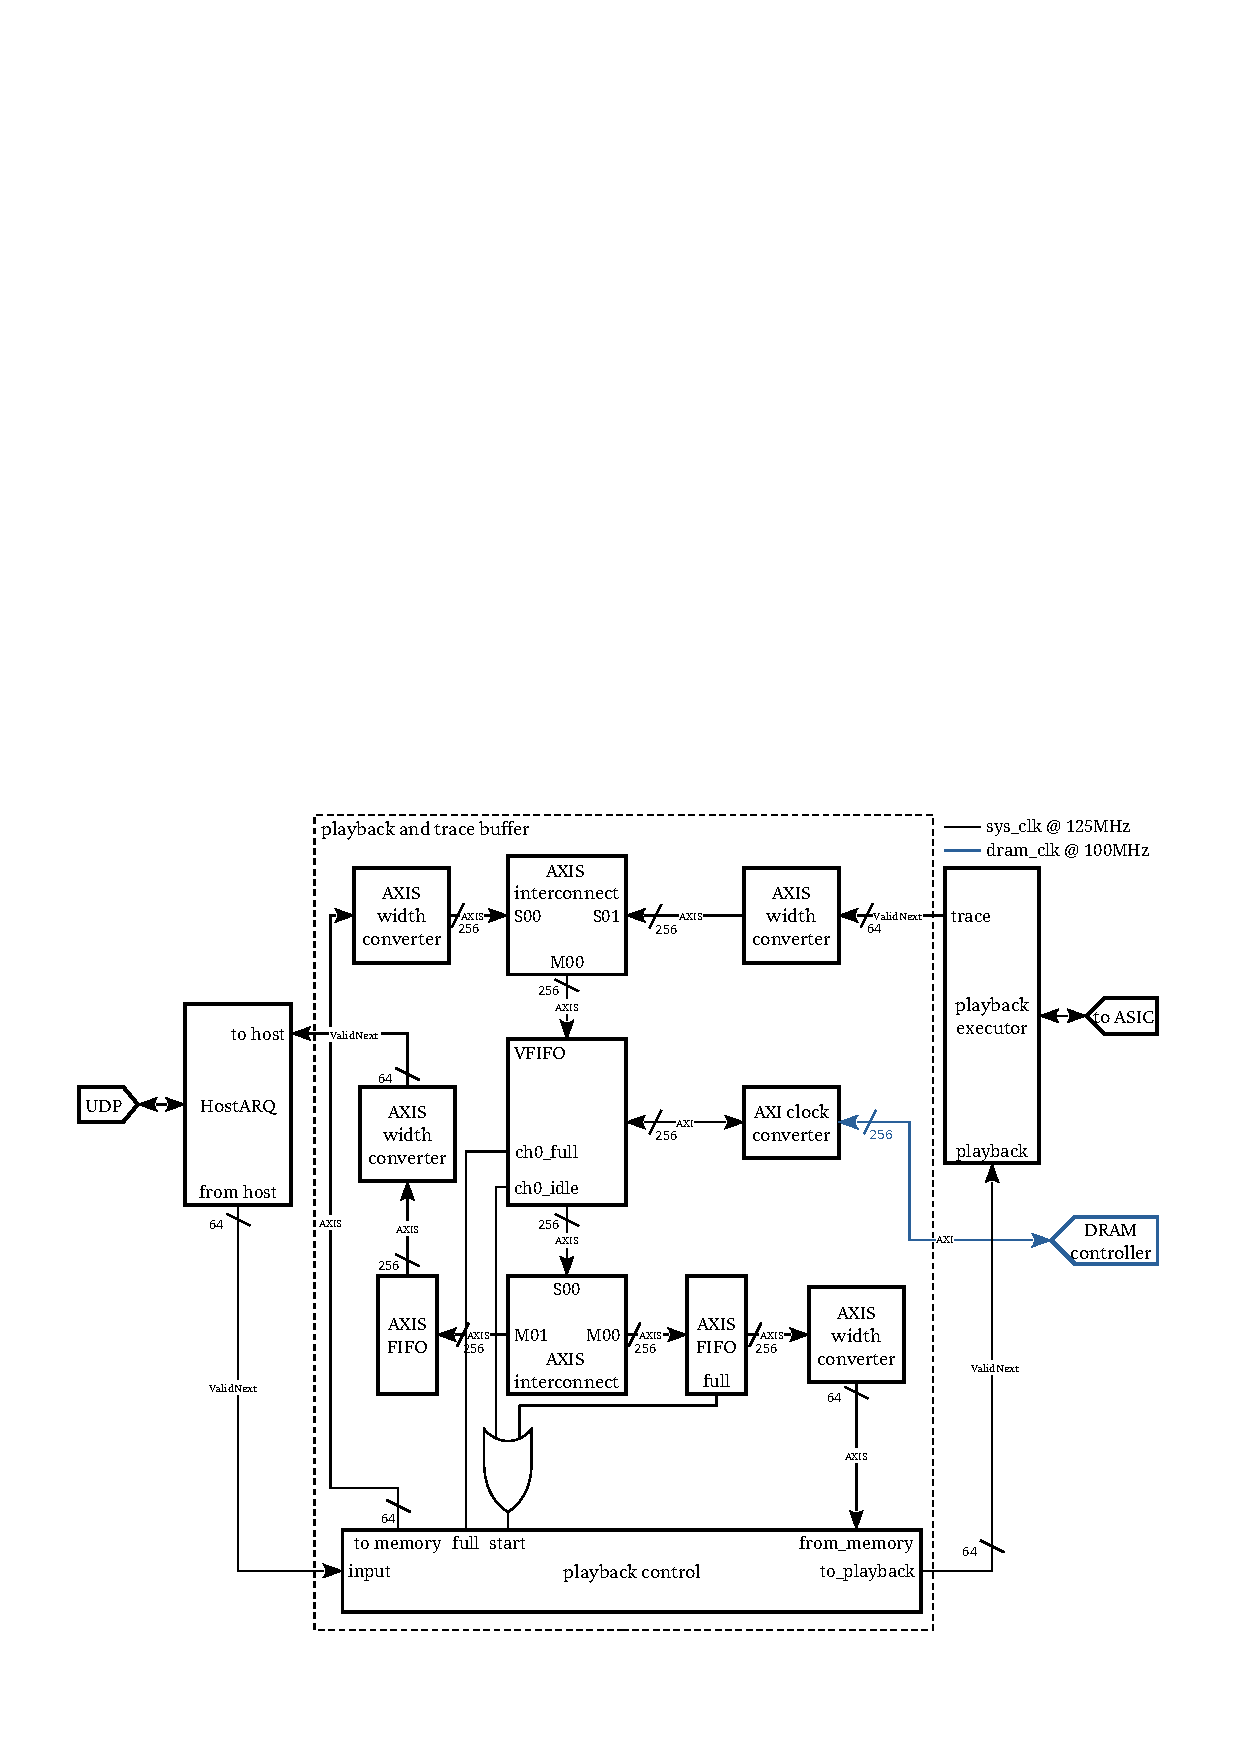
\includegraphics{diagrams/cropped/detail_old}}
\caption{Schematic overview of the old, FIFO{}-based, module handling the playback and trace data. Data received from the host is bufferd in the \DDR{} memory and gated by the playback control to be transmitted to the \pbexec{} once atleast one complete \PlaybackProgram{} was received from the host. In the opposite direction the trace data is stored in the \DDR{} memory until it is transmitted to the host.}\label{diagram:detail_old}
\end{figure}


This implementation of the playback and trace buffer has several shortcomings:
\begin{enumerate}
  \item It can on only use \(\SI{64}{\mebi\byte}\) (\(\SI{32}{\mebi\byte}\) for the playback and \(\SI{32}{\mebi\byte}\) for the trace data) of the available $\SI{512}{\mebi\byte}$ of memory\label{point:limited_size}
  \item The \FIFO{} interface prohibits reading a non contiguous block of the received trace data
  \item The \FIFO{} interface precludes already transmitted \PlaybackProgram{} or parts of them to be reused.
  \item Allocation of the total memory to either playback memory or trace memory is fixed, changing the size of memory allocated to each of them requires generating a new \FPGA{} bitstream.
\end{enumerate}
The maximum size of the two \VFIFO{} channels can be increased by increasing the burst size and allocated pages up to a maximum of \(\SI{256}{\mebi\byte}\) (See table 4-1 in \autocite{ref:vfifo}), which is still only half of the total size of the memory.

A replacement for the playback and trace buffer should fulfill the following requirements
\begin{itemize}
  \item Use the complete $\SI{512}{\mebi\byte}$ of available memory.
  \item Support the maximum possible data rate of $\pbExecBandwidth{}$ supported by the \pbexec{} when transferring the playback data from the memory to the \pbexec{}.
  \item Support the maximum possible data rate of $\pbExecBandwidth{}$ supported by the \pbexec{} when transferring the trace data from the \pbexec{} to the memory.
  \item Allow reuse of already transmitted playback instructions.
  \item Allow out of order access to the received trace data.
\end{itemize}
